\newpage
\section{Introduction}
LLM 属于算法.

\subsection{Computing}
计算是什么? 通过图灵机定义. 

\subsection{Algorithm}
\begin{definition}
    An algorithm $A$ is a procedure that takes an input $I$ and produces an output $O$. (Must terminate)
    \begin{align*}
        A(I)=O
    \end{align*}
\end{definition}
A procedure can go on forever. 无法确认一个程序是否停机(停机问题).

\subsubsection{Russell's Paradox}
罗素悖论(自指)

A town has only one male barber. A man is shaved by the barber if he does not shave himself. Dose the barber shave himself?

Let $S(x)=$ set of people shaved by $x$, so $S(barber)=\{ x|x\notin S(x) \}$.\\
If $barber \notin S(barber)$, then $barber \in S(barber)$. \\
If $barber \in S(barber)$, then $barber \notin S(barber)$. 

\begin{definition}
    A procedure $P$ is an algorithm if $P$ takes any input (binary encoding) always stops and output ``yes'' or ``no''.
\end{definition}
然后就是形式化的罗素悖论: Define an ``algorithm'' $P_k$
\begin{itemize}
    \item Input: Any algorithm $P$ (binary encoding)
    \item Output: 
    \subitem No if $P(P)=$ Yes
    \subitem Yes if $P(P)=$ No
\end{itemize}
$P_k$ is barber, $P$ are other.

\subsection{Undecidable Problems}
不可判定问题. 就是一个判定问题, 被证明没有算法可以判定它. 

\subsubsection{Post Corresponding Problem}
PCP 问题. 

给一些多米诺.

目标: 寻找有限的多米诺, 让上下的字符串一致.

\begin{figure}[!htb]
    \centering
    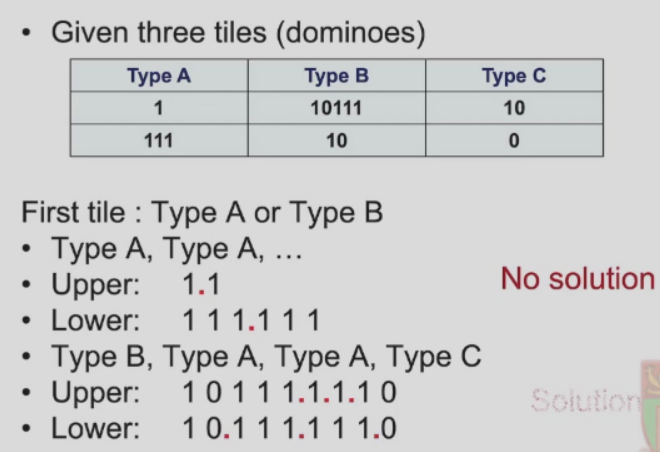
\includegraphics[width=0.309\textwidth]{pic/DAA1/PCP.png}
    \caption{PCP example}
\end{figure}


\subsubsection{Other Undecidable Problem}
\begin{itemize}
    \item Wang tiles
    \item Hilbert's tenth problem
\end{itemize}

\subsection{Algorithm Evaluation}
目标:
\begin{itemize}
    \item 高质量低花销
    \item 最坏情况分析(上界)
    \item 平均情况分析(给输入更多的约束)
\end{itemize}

\subsubsection{Running Time}
\begin{definition}
    Running time: 
    \begin{itemize}
        \item the number of ``primitive/key/basic'' operations or ``steps''. 
        \item function of the input size 
    \end{itemize}
\end{definition}
Input size: number of itmes/bits

关键操作是指无法通过技巧消除的操作. e.g. 线性搜索算法中, 确认是否找到的比较操作就无法去除, 是关键操作. 

\subsubsection{Example Sort}
构建 decision tree, 建模任意的 sort 算法. 

\begin{figure}[!htb]
    \centering
    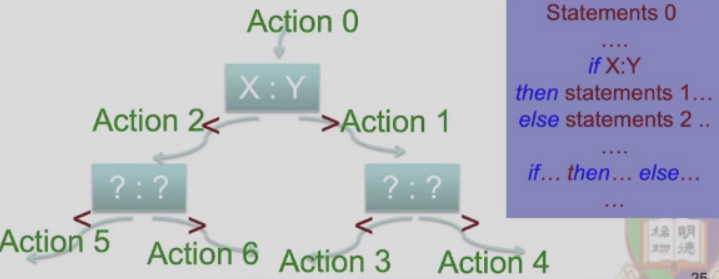
\includegraphics[width=0.42\textwidth]{pic/DAA1/decision tree}
    \caption{decision tree}
\end{figure}

两次比较只能区分出四个排列(permutation). 所以排序 $n$ 个元素, 有
\begin{itemize}
    \item $n!$ 个排列
    \item 下界, decision tree 的高度 $\left\lceil \log_2 n! \right\rceil$. 
\end{itemize} 

\begin{figure}[!htb]
    \centering
    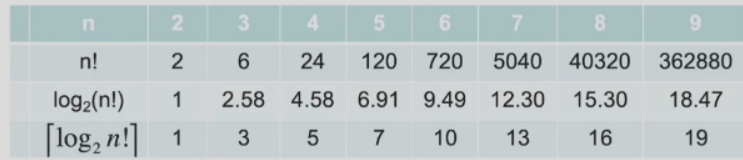
\includegraphics[width=0.42\textwidth]{pic/DAA1/optimal.png}
    \caption{optimal sort}
\end{figure}

\paragraph{在7次比较之内排序5个元素} 并不简单, 因为平常的比较式需要8次. 然后就是一个论文专门讲了这个算法. 第二步比较的应该是 $a_4$

\begin{figure}[!htb]
    \centering
    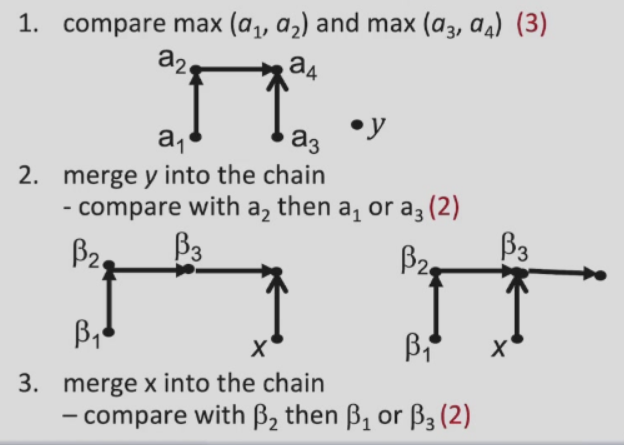
\includegraphics[width=0.42\textwidth]{pic/DAA1/sort5in7}
    \caption{sort 5 in 7}
\end{figure}


\subsubsection{Merge Insertion Sort}
主要思想: 将元素合并到有序链中. 

\begin{figure}[!htb]
    \centering
    \begin{subfigure}{0.42\textwidth}
        \centering
        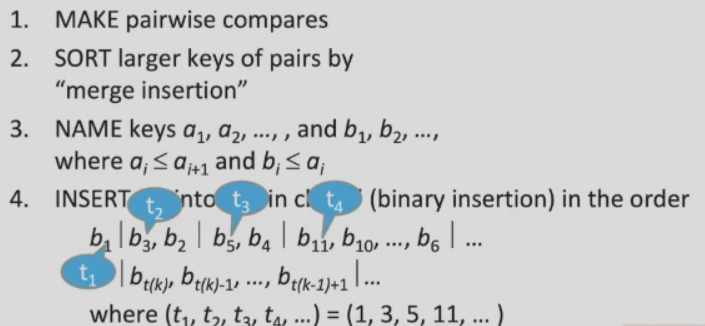
\includegraphics[width=\textwidth]{pic/DAA1/Merge Insertion Sort1}
        % \caption{}
    \end{subfigure}
    \begin{subfigure}{0.42\textwidth}
        \centering
        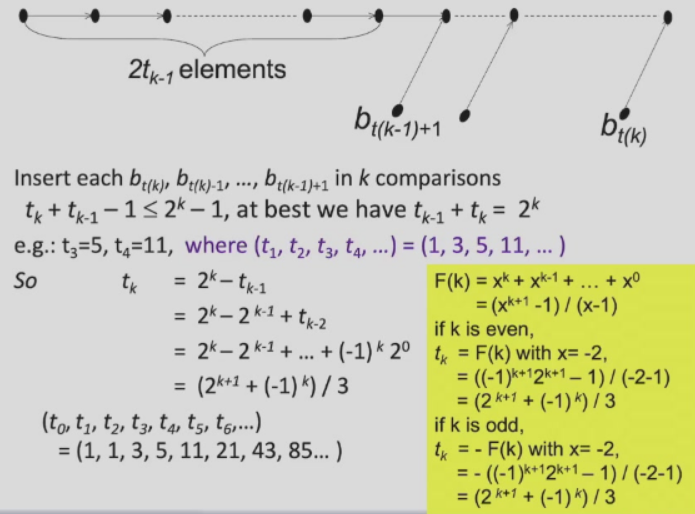
\includegraphics[width=\textwidth]{pic/DAA1/Merge Insertion Sort2}
        % \caption{}
    \end{subfigure}
    \caption{Merge Insertion Sort}
\end{figure}

\paragraph{Time Complexity} of Merge Insert
\begin{figure}[!htb]
    \centering
    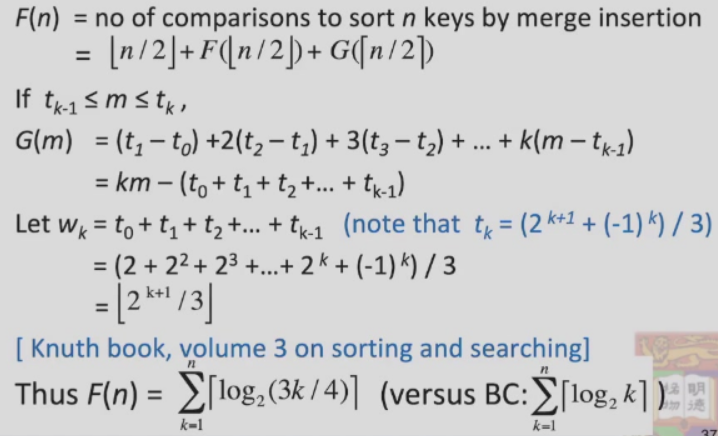
\includegraphics[width=0.42\textwidth]{pic/DAA1/Time Complexity}
    \caption{Time Complexity}
\end{figure}

\subsection{Lower Bound}
下界和问题有关. 算法复杂度不可能小于下界. 若复杂度达到下界, 算法就是最优的. 但即使算法是最优的, 也可能复杂度大于下界. 

Techniques:
\begin{itemize}
    \item decision tree
    \item Adversary(Oracle)
\end{itemize}

\subsubsection{Adversary Argument(Oracle)}
\begin{definition}[Adversary]
    A strategy to create situation to make the algorithm to work hard (releasing the least information and changing scenario).
\end{definition}

为问题建立最坏的情况. 

